\testCom
{%Номер задачи
	3.211
}
{%Условие
	условие
}
{%Дано
	дано
}
{%Найти
	найти
}
{%Решение
	%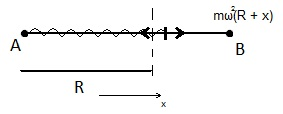
\includegraphics[height=30mm]{3_33.jpg}\\
	Так как стержень закреплён в середине, то свободные концы должны быть пучностями:\\
	$\frac{1}{2} l = n \frac{\lambda}{2} + \frac{\lambda}{4} = \frac{\lambda}{2} (n + \frac{1}{2}), \quad \nu_c = \frac{\upsilon}{\lambda} = \sqrt{\frac{E}{\rho}} \cdot \frac{(n + \frac{1}{2})}{l}$\\
}

